\documentclass[2pt]{article}
\usepackage{amsmath,amsthm,amssymb,geometry,graphicx,wrapfig}
\usepackage[font={small,it}]{caption}
\title{Harmonic Number}
\begin{document}
\date{\vspace{-5ex}}
\maketitle
\section{Introduction}
\begin{wrapfigure}{r}{8cm}
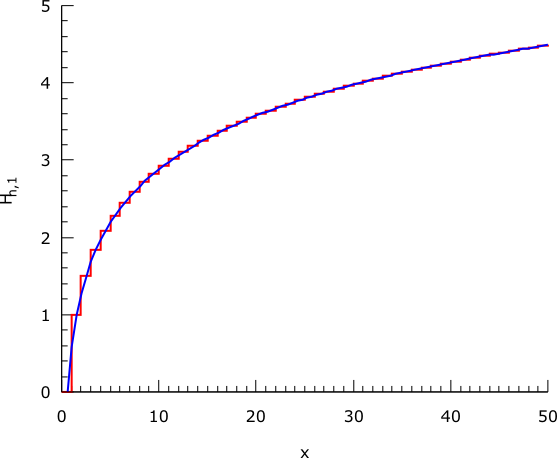
\includegraphics[width=8cm]{1.png}\caption{\small{The harmonic number $H_{n,1}$ with $n=\lfloor{x}\rfloor$ (red line) with its asymptotic limit $\gamma+\ln(x)$ (blue line).}}\end{wrapfigure}
\begin{flushleft}
The term \emph{Harmonic number} has multiple meanings.
\end{flushleft}
In mathematics, the n-th harmonic number is the sum of the reciprocals of the first n natural numbers:
\begin{equation}
H_{n}=1+\frac{1}{2}+\frac{1}{3}+...+\frac{1}{n}=\sum_{i=1}^n \frac{1}{n} \label{nth harmonic number}
\end{equation}

This also equals n times the inverse of the \emph{harmonic mean} of these natural numbers.\\
Harmonic numbers were studied in antiquity and are important in various branches of number theory. They are sometimes loosely termed harmonic series, are closely related to the Riemann zeta function, and appear in the expressions of various special functions.\\
The associated harmonic series grows without limit, albeit very slowly, roughly approaching the natural logarithm function. In 1737, Leonhard Euler used the divergence of this series to provide a new proof of the infinity of prime numbers. His work was extended into the complex plane by Bernhard Riemann in 1859, leading directly to the celebrated Riemann hypothesis about the distribution of prime numbers.\\
When the value of a large quantity of items has a Zipf's law distribution, the total value of the n most-valuable items is the n-th harmonic number. This leads to a variety of surprising conclusions in the Long Tail and the theory of network value.\\
Bertrand's postulate entails that, except for the case n=1, the harmonic numbers are never integers.
\\
\section{Identities involving harmonic numbers}
By definition, the harmonic numbers satisfy the \emph{recurrence relation}
\begin{equation} 
H_{n}=H_{n-1}+\frac{1}{n} \label{recurrence relation}
\end{equation}
They also satisfy the series Identity
\begin{equation}
\sum_{k=1}^n H_{k} = (n+1) H_{n} - n \label{Series Identity}
\end{equation}
The Harmonic numbers are connected the \emph{Stirling Numbers} of first kind
\begin{equation}
H_{n} = \frac{1}{n!} {n+1 \choose 2} \label{Stirling Identity}
\end{equation}
The functions
\begin{equation}
f_{n} (x) = \frac{x^n}{n!} (\log{x}-H_{n})
\end{equation}
satisfy the property
\begin{equation}
{f'}_{n} (x) = f_{n-1} (x)
\end{equation}
In particular
\begin{equation}
f_{1} (x) = x(\log{x}-1)       			
\end{equation}
\section{Eulerian Representation}
An integral representation is given by
\begin{equation}
H_{n} = \int_{0}^{1} \frac{1-x^n}{1-x} dx \label{Euler equation}
\end{equation}
The equakity above is obvious by simple algebraic identiy
\begin{equation}
\frac{1-x^n}{1-x} = 1+x+...+x^{n-1}
\end{equation}
Using a simple integral transform ${x = 1-u}$, an elegant combinatorial expression for $H_{n}$ is
\begin{align}
H_{n} &= \int_{0}^{1} \frac{1-x^n}{1-x} dx \\
	 &= -\int_{1}^{0} \frac{1-{(1-u)}^n}{u} dx \\
	 &= \int_{0}^{1} \frac{1-{(1-u)}^n}{u} dx \\
	 &= \int_{0}^{1} \bigg{[}\sum_{k=1}^{n} (-1)^{k-1} {n \choose k} u^{k-1}\bigg{]}dx \\
	 &= \sum_{k=1}^{n} (-1)^{k-1} {n \choose k} \int_{0}^{1} u^{k-1} dx\\
	 &= \sum_{k=1}^{n} (-1)^{k-1} \frac{1}{k} {n \choose k}
\end{align}
The same repreentation can b produced by using the third \emph{Retkes Identity} by setting $x_{1} = 1, . . . , x_{n} = n$ and using the fact that
\begin{equation}
{\Pi}_{k}(1, . . . , n) = {(-1)}^{n-k} (k-1)!(n-k)!
\end{equation}
\begin{equation}
H_{n}=H_{n,1}=\sum_{k=1}^{n} \frac{1}{k} = {(-1)}^{n-1}n!\sum_{k=1}^{n}\frac{1}{k^{2}{\Pi}_{k}(1, . . . ,n)}=\sum_{k=1}^{n}{(-1)}^{k-1}\frac{1}{k}{n \choose k}
\end{equation}
\begin{wrapfigure}{r}{6cm}
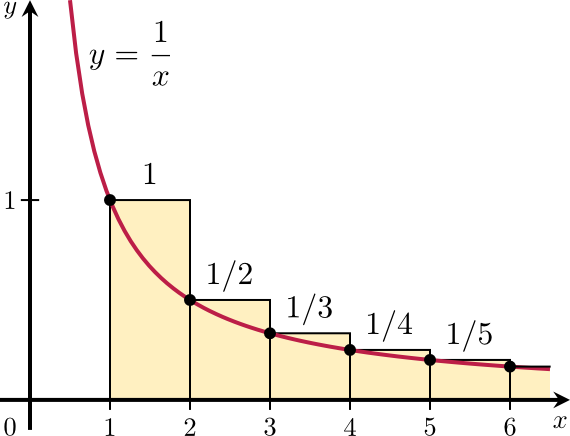
\includegraphics[width=6cm]{2.png}
\caption{\small{Graph demonstrating a connection between harmonic numbers and the natural logarithm. The harmonic number $H_{n}$ can be interpreted as a Riemann sum of the integral: $\int_1^{n+1} \frac{1}{x} \mathrm{d}x = \ln(n+1)$}}
\end{wrapfigure}
The $n^{th}$ harmonic number is about as large as the \emph{natural logarithm} of $n$. The reason is that the sum is approxiamted by the integral
\begin{equation}
\int_{1}^{n} \frac{1}{x} dx
\end{equation}
whose value is \emph{ln(n)} \\
The values of the sequence $H_{n} - ln(n)$ decreases mootonically towards the \emph{limit}
\begin{equation}
\lim_{n \to \infty} (H_{n} - ln(n)) = \gamma
\end{equation}
where $\gamma \sim 0.5772156649$ is the \emph{Euler-Mascheroni Constant}. The correspondng \emph{asymptotic expansion} as $n \to \infty$ is
\\\\\\
\begin{equation}
H_{n} \sim ln \emph{n} + \gamma + \frac{1}{2n}-\sum_{k=1}^{\infty} \frac{B_{2k}}{skn^{2k}}=ln \emph{n} + \gamma + \frac{1}{2n} - \frac{1}{12n^2}+\frac{1}{120n^4}-...
\end{equation}
where $B_{k}$ are the \emph{Bernoulli Numbers}.
\end{document}













